\documentclass{beamer}

\setbeamertemplate{navigation symbols}{}
\setbeamertemplate{footline}{\insertpagenumber}
% This file is a solution template for:

% - Giving a talk on some subject.
% - The talk is between 15min and 45min long.
% - Style is ornate.



% Copyright 2004 by Till Tantau <tantau@users.sourceforge.net>.
%
% In principle, this file can be redistributed and/or modified under
% the terms of the GNU Public License, version 2.
%
% However, this file is supposed to be a template to be modified
% for your own needs. For this reason, if you use this file as a
% template and not specifically distribute it as part of a another
% package/program, I grant the extra permission to freely copy and
% modify this file as you see fit and even to delete this copyright
% notice.


\mode<presentation>
{
  %\usetheme{Warsaw}
  %\usetheme{Montpellier}
  \usetheme{Singapore} % Malmoe}
  % or ...

  \setbeamercovered{transparent}
  % or whatever (possibly just delete it)
}

\input{header}
\usepackage[english]{babel}
% or whatever

\usepackage[mathletters]{ucs}
\usepackage[utf8x]{inputenc}

\usepackage{times}
\usepackage[T1]{fontenc}


% Or whatever. Note that the encoding and the font should match. If T1
% does not look nice, try deleting the line with the fontenc.

\usepackage{tikz}
\usepackage{pgflibrarysnakes}
\usepackage{url}

%% Define a new 'leo' style for the package that will use a smaller font.
\makeatletter
\def\url@leostyle{%
  \def\UrlFont{\sf\footnotesize}}
\makeatother
%% Now actually use the newly defined style.
\urlstyle{leo}

\title[OOP]
{Object-Oriented Programming}

\subtitle{} %
%{OOP} % (optional)


\author[Jean-Philippe Bernardy] % (optional, use only with lots of authors)
{Sibylle Schupp\inst{2} \\
Jean-Philippe Bernardy\inst{1}}
% - Use the \inst{?} command only if the authors have different
%   affiliation.

\institute[Universities of Somewhere and Elsewhere] 
% (optional, but mostly needed)
{
  \inst{1}%
  Department of Computing Science\\
  Chalmers University of Technology\\
  \inst{2}%
  Institute for Software Systems\\
  Hamburg University of Technology
}
% - Use the \inst command only if there are several affiliations.
% - Keep it simple, no one is interested in your street address.

\date%[Short Occasion] % (optional)


\subject{Talks}
% This is only inserted into the PDF information catalog. Can be left
% out.



% If you have a file called "university-logo-filename.xxx", where xxx
% is a graphic format that can be processed by latex or pdflatex,
% resp., then you can add a logo as follows:

\pgfdeclareimage[height=0.5cm]{university-logo}{../../../project/gitroot/clipart/ChalmGUmarke.pdf}
 \logo{\pgfuseimage{university-logo}}



% Delete this, if you do not want the table of contents to pop up at
% the beginning of each subsection:
\AtBeginSubsection[]
{
  \begin{frame}<beamer>
    \frametitle{Outline}
    \tableofcontents[currentsection,currentsubsection]
  \end{frame}
}
\AtBeginSection[]
{
  \begin{frame}<beamer>
    \frametitle{Outline}
    \tableofcontents[currentsection]
  \end{frame}
}

\begin{document}
\begin{frame}
  \titlepage
\end{frame}

\begin{frame}[fragile]
\frametitle{References}
References:
\begin{itemize}
\item M. Scott, Programming Language Pragmatics

\url{http://www.cs.rochester.edu/u/scott/254/notes/09-objects}
\item K. Loudon, Programming Languages---Principles and Practice
(not on-line available)
\end{itemize}

Additional reading:
\begin{itemize}
\item B. Ryders, Univ. Rutgers
\url{
http://remus.rutgers.edu/cs314/s2004/ryder/lectures/adt-15Newest-2up.pdf
}
%
\item K. Bruce, Williams College
\url{
http://www.cs.williams.edu/~kim/cs334/s00/Lectures/Lec13/Lec13.html}
\end{itemize}
\end{frame}

\mycomment {
\begin{frame}[fragile]
\frametitle{Premier (academic) conferences}
\framesubtitle{}

OOPSLA
\begin{itemize}
\item Object-Oriented Programming, Systems, Languages, and Applications
\item 2007: 21th Conference (ACM)
\item \url{http://www.oopsla.org}
\end{itemize}

ECOOP
\begin{itemize}
\item European Conference on Object-Oriented Programming
\item 2007: 22nd Conference (ACM)
\item \url{http://www.ecoop.org}
\end{itemize}

Turing award
\begin{itemize}
\item Ole-Johan Dahl, Kristen Nygaard (Simula), 2001
\item Alan Kay (Smalltalk), 2003
\end{itemize}
\end{frame}
}

\begin{frame}[fragile]
\frametitle{A short history}
\url{http://heim.ifi.uio.no/~kristen/FORSKNINGSDOK_MAPPE/F_OO_start.html}
%Scott, p.788
First generation
\begin{itemize}
\item SIMULA1 (1962-65), SIMULA 67 (1967): 
\begin{itemize}
\item Ole-Johan Dahl, Kristen Nygaard, Oslo
\item Inheritance, virtual methods
\end{itemize}
\item Smalltalk (1969-80) 
\begin{itemize}
\item Alan Kay, Dan Ingalls, Adele Goldberg at Xerox Parc
\item Dynamic language %(dynamic typing)
\end{itemize}
\end{itemize}

80s
\begin{itemize}
\item \cpp(1983-98)
%\begin{itemize}
%\item 
B. Stroustrup, AT\&T; hybrid
%\end{itemize}
\item Eiffel (1986-98); B. Meyer, ISI; %design by contract

\end{itemize}

And later many more:
\begin{itemize}
\item BETA
\item CLOS, Dylan, Cecil, SELF, Ruby, \ldots
\item  Modula-3, Oberon, Ada95, Sather, \ldots
\item Objective CAML, Objective-C, \ldots
\item Java (1995-03),
C\# (2000-03)


\end{itemize}

\end{frame}




\begin{frame}
  \frametitle{Outline}
  \tableofcontents
  % You might wish to add the option [pausesections]
\end{frame}

\section{A Quick Tour through Smalltalk}

\begin{frame}[fragile]
\frametitle{Smalltalk}
Material:
\begin{itemize}
  \item \url{http://www.squeak.org/Smalltalk}
  \item \url{http://squeakbyexample.org/SBE.pdf}
\end{itemize}

Principles
\begin{itemize}
\item Everything is an object.
\item All computation happens by sending \textit{messages} to objects:
\begin{cplus3}
      anObj aMethod: anArg
\end{cplus3}
\item Every object is an instance of a class.
\item All classes have a parent; \texttt{Object} is the root class.
\item All methods are public, all instance variables are private.
\end{itemize}


\end{frame}

\begin{frame}[fragile]
\frametitle{Smalltalk syntax}
% \url{http://www.mucow.com/squeak-qref.html} -- down
\begin{itemize}
\item Assignment
\begin{cplus3}
foo := 100 factorial.
\end{cplus3}

\item Messages
\begin{itemize}
\item Unary
\begin{cplus3}
4 factorial
'bla' asUppercase
Color yellow
\end{cplus3}

\item Infix syntax (``Binary'')
\begin{cplus3}
3 + 4
1 <= 10
3 + 4 * 2
\end{cplus3}

\item Named Arguments (``Keywords'')
\begin{cplus3}
nums := Array newFrom: (1 to: 5)
nums at: 1 put: \$a
nums at: 2 put: 3 + 4
\end{cplus3}
\end{itemize}
\end{itemize}
\end{frame}

\begin{frame}[fragile]
\frametitle{Blocks}
%http://daitanmarks.sourceforge.net/or/squeak/squeak_tutorial.html
Blocks %(a.k.a. block closure) 
correspond to anonymous functions. 

\begin{itemize}
\item They are objects (instances of \texttt{BlockContext}) and
typically receive the message \texttt{value:}.
\item They can have parameters (indicated by a leading colon):

\begin{cplus3}
[:x | 1 + x] value: 2
[:x :y | x + y] value: 1 value: 2
\end{cplus3}

\item They can  have local variables (indicated by bars):
\begin{cplus3}
[:x :y |  |z| z := x + y] value: 1 value:2 
\end{cplus3}

\item They can refer to variables of the surrounding scope
(they create \emph{closures}):
\begin{cplus3}
|newArray|
newArray :=  ... 
[:i | newArray at: i put: (aCollection at: i)]
\end{cplus3}
\end{itemize}

exercise: relate to λ-expression
\end{frame}


\section{Abstract Data Types}
% Loudon, ch. 9

\begin{frame}[fragile]
\frametitle{Motivation}
\framesubtitle{}
Built-in types:
\begin{itemize}
\item abstract from the underlying implementation, 
\item come with a set of predefined operations with predefined semantics
(language specification, mathematics, \ldots).
\item \emph{idealized} classes
\end{itemize}
\bigskip

Suppose users define new types via record-constructors only: 
\begin{cplus2}
       typedef struct {
          int   no_of_edges;
          float edge_size;
       } regular_polygon;
\end{cplus2}
Properties of \textit{such} user-defined types:
\begin{itemize}
\item the underlying implementation is visible,
\item no operations  (directly) associated. 
\end{itemize}
\bigskip

What additional constructs could be provided so that user-defined types
have the same properties as built-in types?

\end{frame}

\begin{frame}[fragile]
\frametitle{Abstract Data Types (ADTs), informally}
\framesubtitle{}
Properties: 

\begin{enumerate}
\item The data type and its operations are defined 
together, in one place, and so that
\begin{enumerate}
\item the operations do not depend on the implementation,
\item their definition includes a specification of their semantics.
\end{enumerate}
\item The implementation of the type and the implementation methods
are defined in one place and so that 
\begin{itemize}
\item clients of the ADT have
limited access only. 
\end{itemize}
\end{enumerate}
\bigskip

Software-engineering advantages:
\begin{itemize}
\item Reuse, maintenance, safety % rethink
\end{itemize}
\end{frame}

\begin{frame}[fragile]
\frametitle{ADT and OOP}
\framesubtitle{}
Object-oriented programming supports ADTs, but ADTs
can also be defined in other paradigms.
\bigskip

Implementation of ADTs: 
\begin{itemize}
\item Classes
\begin{itemize}
\item See next chapter
\end{itemize}

\item Modules
\begin{itemize}
\item Ada package, modules in CLU, Haskell, ML, \ldots
\end{itemize}

\item Special constructs
\mycomment{
\begin{cplus3}
(* ADT SET in ML *)
abstype 'a set = SET of 'a list with
    val empty = SET(nil)
    fun insert(x, SET(elts)) = ...
    fun union(SET(elts1), Set(elts2)) = ...
    fun isMember(x, SET(elts)) = ...
end
\end{cplus3}
}
\begin{cplus3}
(* ADT complex in ML *)
abstype complex = C of real * real with
    fun complex(x,y: real) = C(x,y)
    fun x_coord(C(x,y)) = x
    fun y_coord(C(x,y)) = y
    fun add(C(x1,y1), C(x2,y2)) = C(x1+x2, y1+y2)
end
\end{cplus3}
\end{itemize}

Yet, the specification of an ADT is language-independent:
\begin{itemize}
\item Algebraic specification 
\end{itemize}
\end{frame}

\begin{frame}[fragile]
\frametitle{Algebraic specifications}
\framesubtitle{Overview}

\begin{itemize}
\item Mathematical, language-independent specification of abstract data types.
\item Implementation: not a concern
\end{itemize}

Applications:
\begin{itemize}
\item Language and (abstract) data type design
\item Software specification
\end{itemize}

What?
\begin{itemize}
\item Syntax (operations)
\item Semantics (axioms)
\end{itemize}


\end{frame}

\begin{frame}[fragile]
\frametitle{Algebraic specification}
\framesubtitle{Syntax}

Syntactic specification (``signature''):
\begin{itemize}
\item Name of the ``sort''
\item Operations: name, parameter sorts, return sort
\end{itemize}
\bigskip

Example:
\begin{tabular}{lll}
\multicolumn{3}{l}{\textbf{sort} IntContainer \textbf{imports} integer}\\
\multicolumn{3}{l}{\textbf{operations:}}\\
 & \ \ & 
   \begin{tabular}{ll}
   create:& IntContainer\\
   insert:& IntContainer × integer × integer → IntContainer\\
   remove:& IntContainer × integer → IntContainer \\
   \end{tabular}
\end{tabular} 
\bigskip


Q: what is ``integer''?

The signature defines a language of valid expressions.


\end{frame}


\begin{frame}[fragile]
\frametitle{Algebraic specification}
\framesubtitle{Semantics}
What ''is'' remove? Equations describe the semantic properties of operations.
 They are often called
``axioms.''
\bigskip

Example:
\begin{tabular}{lll}
\multicolumn{3}{l}{\textbf{sort} IntContainer \textbf{imports} integer}\\
\multicolumn{3}{l}{\textbf{operations:}}\\
 & \ \ & 
   \begin{tabular}{ll}
   create:& IntContainer\\
   insert:& IntContainer × integer × integer →  IntContainer\\
   remove:& IntContainer × integer →  IntContainer \\
   \end{tabular} \\
\multicolumn{3}{l}{\textbf{variables:}}\\
& \ \ & 
   \begin{tabular}{l}
    A: IntContainer; i,j,k: integer;
      \end{tabular} \\
\multicolumn{3}{l}{\textbf{axioms:}}\\
& \ \ & 
   \begin{tabular}{l}
   remove(create,i) = create \\
   remove(insert(A,i,j), k) = if i == k then j else remove(A,k) \\
   ...
   \end{tabular}
\end{tabular} 
\bigskip

An ADT must respect the axioms!

% Conditional equational logic frequent; other logics possible.

\end{frame}

\begin{frame}[fragile]
\frametitle{Initial algebras}
\framesubtitle{From algebraic specification to ADTs}
Goal: construct a type which is a model for the spec.
\bigskip

One can proceed as follows (informally):
\begin{itemize}
\item Consider all syntactically valid terms. This is sometimes
called the ``free algebra''.
Ex.:
\\
\hspace*{0.5cm}
{\small\em
\begin{tabular}{l}
create, insert(create,1, 1), 
insert(create,1,2), insert(create,2,1),\\
insert(insert(create,1,1),2,2), remove(insert(create,1,1), 1), \ldots
\end{tabular}
}
This surely contains ``enough'' values: if you can write the expression, you
can find it in there!

\item The above contains ``too much'': the axioms are not respected.
(Ex. remove(create,0) ≠ create ...) 

\item The ``initial algebra'' is a subset of the ``free algebra''.
  Additionally, if one can prove $x=y$ using the axioms, then $x$ and $y$ are
  considered the same element.
\end{itemize}
\end{frame}

\mycomment{
\begin{frame}[fragile]
\frametitle{Final algebras}
\framesubtitle{From algebraic specification to ADTs (alternative)}

Different representations 
(of axioms) and the order of operations lead to different initial algebras.
This could be too strict.
\bigskip

Final algebra:
\begin{itemize}
\item Proceed as with initial algebras, but construct quotient
algebra using equivalence relation
\begin{center}
  $x == y$ iff the values of $x,y$ \textit{cannot be distinguished}.
\end{center}

\end{itemize}
Difference to initial algebra:
\begin{center}
\hspace*{0.5cm}
{\small\em
\begin{tabular}{l}
insert(insert(create,1,1),2, 2), 
\end{tabular}
}
and 
{\small\em
\begin{tabular}{l}
insert(insert(create,2,2), 1,1), 
\end{tabular}
}
\end{center}

are equal in the final algebra but not in the initial algebra.
\bigskip

Final algebras do not always exist.

\end{frame}
} % end mycomment

\mycomment{
\begin{frame}[fragile]
\frametitle{Formal language}
\framesubtitle{}
%
Specifications themselves can be based on languages: 
\textit{formal}  languages. 
\bigskip

\begin{itemize}
\item Automated checks possible!
\item Many (algebraic) specification languages exist: CASL, COFI,
OBJ family, Larch family, Tecton, Lotus, LPG, \ldots
% JML, etc.
\item Principal problem: gap to programming language 
\end{itemize}
\end{frame}
}

\mycomment{
\begin{frame}[fragile]
\frametitle{\Cpp concepts}
\framesubtitle{On the cutting edge}

\begin{itemize}
\item  \cpp extension by a specification language (``concepts'')
% \item Proposal approved by the evolution group $\leadsto$ \cpp0x
\item Combines advantages:
\begin{itemize} 
\item specification (formal \& implementation-independent), \\ 
but \textit{within the language/tool chain} 
\end{itemize}
\item Experimental compiler exists (ConceptGCC).



%http://www.generic-programming.org/languages/conceptcpp/concept_web.php
\begin{cplus3}
// From http://www.generic-programming.org/languages/conceptcpp
auto concept EqualityComparable<typename T, typename U = T> {
   bool operator==(T, U); 
   axiom Reflexivity(T x) { x == x; } 
   axiom Symmetry(T x, T y) {if (x == y) y == x; }
   axiom Transitivity(T x, T y, T z) {if (x == y && y == z) x==z;}
};

concept CopyConstructible<typename T> {
    T::T(const T&);
    axiom CopyEquivalence(T x) {
      T(x) == x; 
   }
}
\end{cplus3}
\end{itemize}
\end{frame}

}

\mycomment {

\begin{frame}[fragile]
\frametitle{Design by contract (TM) in Eiffel}
\framesubtitle{Interface specification of methods}
%http://archive.eiffel.com/doc/online/eiffel50/intro/language/tutorial-09.html

Eiffel provides syntax for expressing  pre- and postconditions of
methods: 
\begin{cplus3}
   --- http://archive.eiffel.com/doc/manuals/technology/contract/
   put (x: ELEMENT; key: STRING) is
             -- Insert x s.t. it will be retrievable through key.
             require
                     count <= capacity
                     not key.empty
             do
                     ... Some insertion algorithm ...
             ensure
                     has (x)
                     item (key) = x
                     count = old count + 1
             end
\end{cplus3}
\begin{itemize}
\item \textit{require} establishes the precondition.
\item \textit{ensure} establishes the postcondition.
%\item
\end{itemize}
%Can you express the postconditions as equations?

\end{frame}


}


\mycomment{
\begin{frame}[fragile]
\frametitle{Encapsulation and information hiding}
\framesubtitle{}
Software-engineering parlance:
\bigskip

\begin{itemize}
\item Encapsulation: 
\begin{itemize}
\item 
group the operations and data related to a data type
in one place, 
\item  include methods for (restricted) access to the type's value 
and ensure that no other access is possible.
\end{itemize}
\item Information hiding: 
\begin{itemize}
\item separate interface and implementation,
\item hide implementation. 
\end{itemize}
\end{itemize} 

\end{frame}
}

\section{Objects}
\begin{frame}[fragile]
\frametitle{What are objects? }
\framesubtitle{}
Objects  are entities with a modifiable state and a set of functions to access
and change that state.
\begin{itemize}
\item The state is local to the object and (meant to be) inaccessible to 
others.
\item The functions have an implicit parameter, the object itself (``this'').
\end{itemize}

Functions in OOP are called \textit{methods} or \textit{messages}.
\bigskip

The local variables of an object are called \textit{instance variables}
or \textit{fields}.
\bigskip

An object \textit{instantiates} a class.
\end{frame}



\begin{frame}[fragile]
\frametitle{What are classes?}
\framesubtitle{}
It is hard to give a definition of the term \textit{class} that holds
for all classes in all OO-languages. 

\bigskip

Some aspects:

\begin{itemize}
\item A class groups the fields and methods of an object.
\item A class is \textit{instantiable} by objects.
It contains \textit{constructors} to allocate and initialize objects.
\item A class is a unit of inheritance: it is derived from another
class and one can use it to derive a new class from it. 
\item A class is a type. 
% in statically-typed languages
\end{itemize}
\bigskip

Most OO-languages permit classes that do not (have to) exhibit 
all aspects. 
\end{frame}

\begin{frame}[fragile]
\frametitle{Next on the agenda}
\framesubtitle{}
\begin{itemize}
\item Methods
\begin{itemize}
\item Multimethods
\end{itemize}
\item Object state
\begin{itemize}
\item Object creation 
\item Deallocation
\end{itemize}

\end{itemize}
\end{frame}

\subsection{Methods}
\begin{frame}[fragile]
\frametitle{Methods}
\framesubtitle{}
If we ignore inheritance (for the moment), class methods  are
quite similar to ``free'' functions. 
\bigskip

Difference:
\begin{itemize}
\item Implicit ``this'' parameter: receiver object 
\begin{itemize}
\begin{cplus3}
// free function 'add'
complex add(const complex& x, const complex& y) {...}

// method 'add'
class complex {
    complex add(const complex& y) {...}
};

\end{cplus3}
\item  Exception: static methods
\end{itemize}
\item Can access the internal state.
\end{itemize}


\end{frame}

\begin{frame}[fragile]
\frametitle{Binary methods}
\framesubtitle{Or more general: n-ary methods}
\begin{itemize}
\item Binary methods  take 2 parameters of the same type.
\item 
In OOP, binary methods are methods that contain one or more parameters
of the same type as the receiver object.
\item Examples: arithmetic, equality, comparison, \ldots
\end{itemize}
\bigskip

They cause great difficulties in OOP. 
\end{frame}

\begin{frame}[fragile]
\frametitle{Binary methods problem}
\framesubtitle{Bruce, Cardelli, Hopkins Object Group }
% typing in the presence of inheritance.

Problem: 

\begin{itemize}
\item Receiver and argument are not treated symmetrically (but
should be). 
\end{itemize}

\bigskip

Other problems (also big): 

\begin{itemize}
\item Retrofitting of new classes not possible (makes extension
impossible)
\item Special access rights needed (violates protection)
%\item Do subclasses always produce subtypes?
\end{itemize}
\end{frame}

\begin{frame}[fragile]
\frametitle{Asymmetry}
\begin{cplus3}
class Complex 
{
    // add: (Complex , Real) -> Complex  
    public Complex add(Real d) {...}
}
\end{cplus3}
How to define an addition with signature 
\begin{center}
\textit{double x Complex} → \textit{Complex}?
\end{center}
\begin{itemize}
\item Impossible in almost all OO-language (Java, C\#)!
Exception: very few (``multi-dispatch languages'') 
\item Possible in hybrid language (Ada, \Cpp) via non-OO constructs,
e.g., free functions and overloading (or ``friends''). 
\end{itemize}
\end{frame}

\begin{frame}[fragile]
\frametitle{Method dispatching}
\framesubtitle{}

Single-dispatch languages
\begin{itemize}
\item Dispatch based on the (dynamic) class of the receiver. 
\begin{cplus3}
     Complex c = ... ;   
     c.add(arg);
\end{cplus3}
\item Ex.: all languages mentioned so far

\end{itemize}

Multiple-dispatch languages
\begin{itemize}
\item Dispatch (also) based on the dynamic class of \textit{arguments}.
\item Ex.: Dylan (Apple), CLOS, Cecil
\item Deviation from previous class concept: data records + generic functions.
\begin{cplus3}
     add(arg1, arg2);
\end{cplus3}
\item Combined overloading \& overriding (resolution at run time).
\end{itemize} 
\end{frame}

\begin{frame}[fragile]
\frametitle{Multi-methods in Dylan}
\framesubtitle{}
A multi-method is a method that does not belong to one class
\begin{itemize}
\item For each binary method, there exists
a set of method bodies associated with the name of the method.
\item The dispatch depends on all parameter types.
\end{itemize}
\begin{cplus3}
// http://www.opendylan.org/books/dpg/db_88.html
// Generic ``+'' 
// Method on <time-offset>, <time-offset>
define method \+
    (offset1 :: <time-offset>, offset2 :: <time-offset>)
=> (sum :: <time-offset>)
 let sum = offset1.total-seconds + offset2.total-seconds;
 make(<time-offset>, total-seconds: sum);
end method \+;	

// Method on <time-offset>, <time-of-day>
define method \+ 
    (offset :: <time-offset>, time-of-day :: <time-of-day>)
 => (sum :: <time-of-day>)
  make(<time-of-day>, 
       total-seconds: offset.total-seconds + time-of-day.total-seconds);
end method \+;
\end{cplus3}
\end{frame}

\subsection{Object state}

\begin{frame}[fragile]
\frametitle{Classes in Simula}
%http://staff.um.edu.mt/jskl1/talk.html#Classes
\framesubtitle{}
A class in Simula consists of 4 parts, called:
%\begin{itemize}
%\item 
parameters, attributes, methods,
and  life (body). 
%\end{itemize}
\bigskip

\begin{cplus3}
! From the overview by J. Sklenar
! http://staff.um.edu.mt/jskl1/talk.html
Class Rectangle (Width, Height); Real Width, Height;
                           ! Class with two parameters;
 Begin
    Real Area, Perimeter;  ! Attributes;

    Procedure Update;      ! Methods (Can be Virtual);
    Begin
      Area := Width * Height;
      Perimeter := 2*(Width + Height)
    End of Update;

    Boolean Procedure IsSquare;
      IsSquare := Width=Height;

    Update;                ! Life of rectangle started at creation;
    OutText("Rectangle created: "); OutFix(Width,2,6);
    OutFix(Height,2,6); OutImage
 End of Rectangle;
\end{cplus3}
\end{frame}

\begin{frame}[fragile]
\frametitle{Classes in  Eiffel}
\framesubtitle{}
\begin{eiffel}
-- se.ethz.ch/teaching/ss2006/0050/slides/eiffel_the_essentials.pdf
indexing 
     description: "Representation of a book" 
class 
     BOOK 
create 
     make 
feature {NONE} -- Initialization 
     make (a_title: like title; some_authors: like authors) is 
          require 
                a_title_not_void: a_title /= Void 
                a_title_not_empty: not a_title.is_empty 
          do 
                title := a_title 
                authors := some_authors 
          ensure 
               title_set: title = a_title 
               authors_set: authors = some_authors 
          end 
feature -- Access 
     title: STRING 
invariant 
     title_not_void: title /= Void 
     title_not_empty: not title.is_empty 
end
\end{eiffel}
\end{frame}



\begin{frame}[fragile]
\frametitle{Constructors and initialization}
Object creation is typically done by constructors. Two tasks:
\begin{itemize}
\item Allocate memory 
\item Initialize fields
\end{itemize}
\framesubtitle{}
%se.ethz.ch/teaching/ss2006/0050/slides/eiffel_the_essentials.pdf 
\bigskip

Syntax (example) of constructors:
\begin{eiffel}
! Simula
Ref(Rectangle) R;
R :- New Rectangle(10,20)

-- Eiffel
b: Book
create b.make(``Another Harry Potter'', ``Rowling'')
\end{eiffel}
\bigskip

More examples: Modula-3 provides no constructors; Ada95 only for 
objects derived from Controlled. \Cpp has default ctors (initialization
not required).
\end{frame}

\mycomment{
\begin{frame}[fragile]
\frametitle{More on constructors}
\framesubtitle{}
Name
\begin{itemize}
\item Predefined as in Java, \Cpp, C\#? Or any name, as in Eiffel?
\end{itemize}
Signature
\begin{itemize}
\item  Multiple constructors possible ($\leadsto$ overloading)? 
\end{itemize}
Definition
\begin{itemize}
\item 
Does the compiler create constructors (``default constructor'')? When? 
Can they be overridden?
\begin{eiffel}
-- Eiffel
default_create is
     do 
         create books.make
     end
// C++
class Point {
    int x, y;
public:
    Point(): x(0), y(0) {}
};    
\end{eiffel}
\end{itemize}
\end{frame}
}

\mycomment{
\begin{frame}[fragile]
\frametitle{Meta-classes in Smalltalk}
\framesubtitle{}
In Smalltalk, only objects can send messages.
What is the object that can send a 'creation' message? 
\begin{itemize}
\item Must belong to a class, but can't be of the same class. 
\end{itemize}
\bigskip

A \textit{meta-class} is a  class whose instances are classes.
\begin{itemize}
\item For every Smalltalk class, there exists a meta-class. The meta-classes
mirror the class hierarchy.
\item They specify how to create objects. 
\\ Examples:
\begin{java}
Time now.
   ``Answer a Time representing the time right now - is a 
     24 hour clock.''
Time new.
   ``Answer a Time representing midnight.''
Date today.
Data firstWeekdayOfMonth.
   ``Answer the weekday index of the first day in <month> 
     in the <year>.

\end{java}

\end{itemize}
\end{frame}
}

\begin{frame}[fragile]

\frametitle{Object models}
\framesubtitle{Layout in memory}
Value model:
\begin{itemize}
\item Variables (fields) stored as values, objects allocated directly
on run-time stack. Ex: \cpp, \textit{struct}s in C\#
%Ada, Modula-3
\end{itemize}

\begin{tabular}{ll}
\begin{minipage}{5cm}
\begin{cplus3}
public struct Poly { // C#
    public int deg;
    public myvector terms;
}
Poly p; 
p.deg = 
\end{cplus3}
\end{minipage}

& 

\begin{tabular}{l}
{\small 
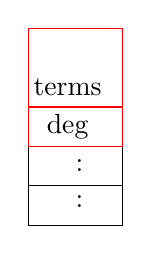
\begin{tikzpicture}
\draw (0,0)  rectangle (1.2,0.5);
\pgftext[at={\pgfpoint{0.65cm}{0.3cm}}]{:} ;
%\draw[->] (1.0, 0.1) .. controls (1.9, -0.2) and (2.5, 2.5) .. (3,1.5);

\draw (0,0.5)  rectangle (1.2,1.0);
\pgftext[at={\pgfpoint{0.65cm}{0.75cm}}]{:} ;


\draw[red] (0,1.0)  rectangle (1.2,1.5);
\pgftext[at={\pgfpoint{0.5cm}{1.25cm}}]{deg} ;


\draw[red] (0,1.5)  rectangle (1.2,2.5);
\pgftext[at={\pgfpoint{0.5cm}{1.75cm}}]{terms} ;

%\draw[red] (0,2.0)  rectangle (1.2,2.5);
%\pgftext[at={\pgfpoint{0.5cm}{1.75cm}}]{} ;


\end{tikzpicture}
}
\end{tabular}
\end{tabular}
%\bigskip

Reference model:
\begin{itemize}
%\item References are stored, object is allocated on the heap.
\item Run-time stacks holds a reference;  object (fields)
allocated on the heap.
Ex: Smalltalk (pure), Java/C\# : class inst's
\end{itemize}


%
\begin{tabular}{ll}
\begin{minipage}{4cm}

\end{minipage}

& 

\begin{tabular}{l}
{\small 
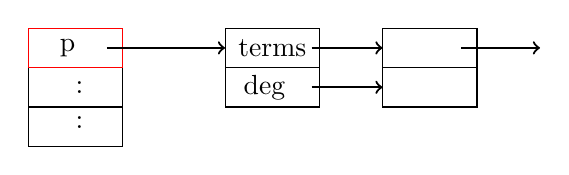
\begin{tikzpicture}
\draw (0,0)  rectangle (1.2,0.5);
\pgftext[at={\pgfpoint{0.65cm}{0.3cm}}]{:} ;
%\draw[->] (1.0, 0.1) .. controls (1.9, -0.2) and (2.5, 2.5) .. (3,1.5);

\draw (0,0.5)  rectangle (1.2,1.0);
\pgftext[at={\pgfpoint{0.65cm}{0.75cm}}]{:} ;


\draw[red] (0,1.0)  rectangle (1.2,1.5);
\pgftext[at={\pgfpoint{0.5cm}{1.25cm}}]{p} ;
\draw[->, thick] (1.0, 1.25) -- (2.5,1.25); 

%\draw (0,1.5)  rectangle (1.2,2.0);
%\pgftext[at={\pgfpoint{0.5cm}{1.75cm}}]{a: 4 } ;



% Object 
%\draw (3,0)  rectangle (4.2,0.5);
%\pgftext[at={\pgfpoint{3.5cm}{0.25cm}}]{prev} ;

\draw (2.5,0.5)  rectangle (3.7,1.0);
\pgftext[at={\pgfpoint{3.0cm}{0.75cm}}]{deg} ;
\draw[->, thick] (3.6, 0.75) -- (4.5,0.75); 
%
\draw (2.5,1.0)  rectangle (3.7,1.5);
\pgftext[at={\pgfpoint{3.1cm}{1.25cm}}]{terms} ;
\draw[->, thick] (3.6, 1.25) -- (4.5,1.25); 

% Object fields
\draw (4.5,0.5)  rectangle (5.7,1.5);
\draw[->, thick] (5.5, 1.25) -- (6.5,1.25); 
\draw (4.5,1.0)  rectangle (5.7,1.5);
%\pgftext[at={\pgfpoint{4.5cm}{1.25cm}}]{x: 3} ;


\end{tikzpicture}
}
\end{tabular}
\end{tabular}

Value model more efficient; reference model more flexible.

\end{frame}


\begin{frame}[fragile]
\frametitle{Curse of temporaries}
\framesubtitle{The costs of OOP}
How many objects are constructed?
\begin{cplus3}
     // C++
     typedef matrix<complex<float> > > matrix;
     matrix M = ...; // construct M
     matrix N = matrix(M);
     M = (M + N) * N;
\end{cplus3}
\bigskip

Intermediate objects (``temporaries'') are a practical problem:
\begin{itemize}
\item Run-time costs
\item Memory costs
\end{itemize}
\bigskip

Advanced techniques exist to avoid their creation.\\
If they must be created, at least  limit their lifetimes.
\end{frame}


\begin{frame}[fragile]
\frametitle{Automated deallocation and destruction}
\framesubtitle{}
Garbage collection
\begin{itemize}
\item Internal routine that automatically visits the heap, looks for
unused (``non-referenced) objects. 
\item Performs necessary finalization
and reclaims the memory.
\end{itemize}
Destructors 
\begin{itemize}
\item 
Based on blocks and scoping mechanisms: deallocation 
done automatically (when object leaves block = ``goes out of scope'').
\item Finalization: encapsulated in destructor. 
Destructor called automatically 
(when object goes out of scope).
\begin{cplus3}
// Example: C++ destructors  
class file {
public:
   file( const string&  name ) : file_handle(fopen(name, "w+")){}  
   ~file() { fclose(file_handle); }  // destructor
private:
   ...
};
\end{cplus3}
\end{itemize}
\end{frame}





\section{Inheritance}


\begin{frame}[fragile]
\frametitle{Subclassing}
\framesubtitle{}
A class is a subclass of another class if it inherits 
its fields and methods.
\bigskip

Syntax (examples)

\begin{cplus3}
    ! Simula
    Rectangle Class LocRectangle (X,Y); Integer X, Y;
    Begin .... 
    End of LocRectangle;

    '' Smalltalk''
    Shape subclass: #Rectangle
        instanceVariableNames: 'width height'
        classVariableNames: ''
        poolDictionaries: ''
        category: ''

     // C# and C++
     public class Rectangle: Shape 
     {
        ... 
     }

\end{cplus3}

\end{frame}


\begin{frame}[fragile]
\frametitle{Object model under inheritance}
\framesubtitle{}
The child object incorporates a parent \textit{object}, i.e., its fields.
(Though it  may not have access to them.)
\bigskip

Value model:

\begin{tabular}{ll}
\begin{minipage}{4cm}
\begin{cplus3}
class base {
   boolean b; 
   poly p;
}
class child extends base {
  integer c;
}
\end{cplus3}
\end{minipage}

& 

\begin{tabular}{l}
{\small 
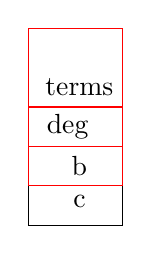
\begin{tikzpicture}
\draw (0,0)  rectangle (1.2,0.5);
\pgftext[at={\pgfpoint{0.65cm}{0.3cm}}]{c} ;
%\draw[->] (1.0, 0.1) .. controls (1.9, -0.2) and (2.5, 2.5) .. (3,1.5);

\draw[red] (0,0.5)  rectangle (1.2,1.0);
\pgftext[at={\pgfpoint{0.65cm}{0.75cm}}]{b} ;


\draw[red] (0,1.0)  rectangle (1.2,1.5);
\pgftext[at={\pgfpoint{0.5cm}{1.25cm}}]{deg} ;


\draw[red] (0,1.5)  rectangle (1.2,2.5);
\pgftext[at={\pgfpoint{0.65cm}{1.75cm}}]{terms} ;

%\draw[red] (0,2.0)  rectangle (1.2,2.5);
%\pgftext[at={\pgfpoint{0.5cm}{1.75cm}}]{} ;


\end{tikzpicture}
}
\end{tabular}
\end{tabular}

\bigskip

Reference model:

\begin{tabular}{ll}
\begin{minipage}{4cm}

\end{minipage}

& 

\begin{tabular}{l}
{\small 
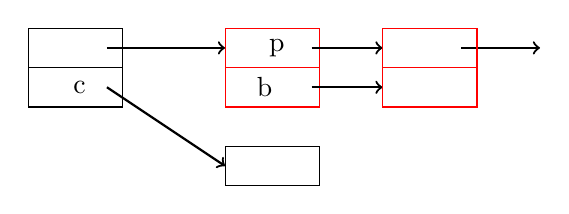
\begin{tikzpicture}
%\draw (0,0)  rectangle (1.2,0.5);
%\pgftext[at={\pgfpoint{0.65cm}{0.3cm}}]{:} ;
%\draw[->] (1.0, 0.1) .. controls (1.9, -0.2) and (2.5, 2.5) .. (3,1.5);

\draw (0,0.5)  rectangle (1.2,1.0);
\pgftext[at={\pgfpoint{0.65cm}{0.75cm}}]{c} ;
\draw[->, thick] (1.0, 1.25) -- (2.5,1.25); 

\draw(0,1.0)  rectangle (1.2,1.5);
\pgftext[at={\pgfpoint{0.5cm}{1.25cm}}]{} ;
\draw[->, thick] (1.0, 0.75) -- (2.5,-0.25); 




% Object 
\draw (2.5,-0.5)  rectangle (3.7,0.0);
\pgftext[at={\pgfpoint{3.0cm}{-0.25cm}}]{} ;

\draw[red] (2.5,0.5)  rectangle (3.7,1.0);
\pgftext[at={\pgfpoint{3.0cm}{0.75cm}}]{b} ;
\draw[->, thick] (3.6, 0.75) -- (4.5,0.75); 
%
\draw[red] (2.5,1.0)  rectangle (3.7,1.5);
\pgftext[at={\pgfpoint{3.1cm}{1.25cm}}]{ p} ;
\draw[->, thick] (3.6, 1.25) -- (4.5,1.25); 

% Object fields
\draw[red] (4.5,0.5)  rectangle (5.7,1.5);
\draw[->, thick] (5.5, 1.25) -- (6.5,1.25); 
\draw[red] (4.5,1.0)  rectangle (5.7,1.5);


\end{tikzpicture}
}
\end{tabular}
\end{tabular}

\end{frame}

\begin{frame}[fragile]
\frametitle{Name clashes of fields }

What if subclass and superclass have a field with the same name?
\begin{itemize}
\item Shadowing: the superclass's field still exists in the subclass but is
\textit{shadowed} by the subclass (most languages).
\item Renaming: resolve the name clash by hand. \\
Eiffel:
\begin{eiffel}
class
   FRIEND
inherit
    PERSON
       rename
           name as legal_name
       end
feature
     name: STRING
end -- class FRIEND

\end{eiffel}
\end{itemize}
%XXX Ruby alias
\end{frame}

\subsection{Refinement, replacement, overriding}
\begin{frame}[fragile]
\frametitle{Methods in subclasses}
\framesubtitle{}
The subclass
\begin{itemize}
\item can use  the methods of the superclass,
\item can add new methods,
\item can ``override'' the methods of the superclass.
\end{itemize}
\bigskip

American vs. Scandinavian semantics of overriding
\begin{itemize}
\item Refinement
\begin{itemize}
\item Parent method executed within the child's method
\item Behavior of the parent method preserved
\end{itemize}
\item Replacement
\begin{itemize}
\item Parent method not executed 
\item Behavior of the parent might or might not be preserved 
\end{itemize}
\end{itemize}
\end{frame}

%\begin{frame}[fragile]
%\frametitle{Refinement in Simula}
%\framesubtitle{}


%\end{frame}


\begin{frame}[fragile]
\frametitle{Refinement in Beta}
\framesubtitle{http://www.daimi.au.dk/~beta/}
When the child method is invoked:
\begin{itemize}
\item At the beginning, control switches to the parent.
\item Parent code starts executing.
\item When 'inner' is encountered, control switches
back to the child. 
\item If there is no child, 'inner' does nothing. 
\end{itemize}
\begin{java}
employee:
(# computeSalary:< 
     (# salary: @integer 
     do noOfHours*80->salary; inner; 0->totalHours  
     exit salary
     #)
#);
worker: employee
    (# computeSalary::< 
       (# do seniority*4+salary->salary; inner #)
 #);

\end{java}

\end{frame}

\begin{frame}[fragile]
\frametitle{Replacement}
\framesubtitle{}
In replacement semantics, a method with ``the same'' signature 
entirely overrides a method in the superclass. 
\bigskip

\begin{java}
public class Parent {	 // Java 
 void printMe () {	  
       System.println(``Parent prints; ``);	 
  }
}
class Child extends Parent { 
    public void printMe () {
       System.println(``Child prints;''); 
    }
}
\end{java}
Design questions:
\begin{itemize}
\item Is overriding done automatically or must the designer
declare overriding?
\item Can refinement semantics be simulated?
\item %What does ``the same'' mean?
What restrictions are placed on argument and return types?
\end{itemize}


\end{frame}

\begin{frame}[fragile]
\frametitle{Overriding in C\#}
\framesubtitle{}
Two keywords in C\#
\begin{itemize}
\item \texttt{virtual} for parent method. 
Parent must agree that method is overridable  (see chapter on dynamic binding).
\item \texttt{override} for child method. 
Child must make explicit that it wants to override. 
\end{itemize}
\begin{java}
// C#
public class Parent {			
   public virtual void printMe () {	  
       System.println(``Parent prints; ``);	 
  }
}
class Child:  Parent { 
    public override void printMe () {
       System.println(``Child prints;''); 
    }
}
\end{java}

C\# also supports hidden methods (keyword: \texttt{new}).

% Eiffel: redefine
\end{frame}

\begin{frame}[fragile]
\frametitle{Pre-and postconditions in Eiffel}
\framesubtitle{Restricting replacement semantics}
\textit{Assertion redeclaration rule}: a redeclared version need not contain its own requires or ensure
clause.
\begin{itemize}
\item It may use a \texttt{require else} or
\texttt{then ensure} clause
to weaken/strengthen the pre/postcondition of the parent. 

\end{itemize}
\begin{eiffel}
class ACCOUNT 
feature
   withdraw(sum: INTEGER) is
       require
           sum >= 0
       do ..  end
end -- class ACCOUNT
class SPECIAL_ACCOUNT inherit
      ACCOUNT
      redefine withdraw end
feature
       withdraw(sum: INTEGER) is
       do ...
       ensure then
           balance >= 1000
       end
end -- class SPECIAL_ACCOUNT       
\end{eiffel}
\end{frame}

\begin{frame}[fragile]
\frametitle{Constructors and refinement semantics}
\framesubtitle{}
Recall the object model: 
\begin{itemize}
\item
the creation of a child object must ensure that its parent is
constructed as well $\leadsto$ refinement semantics!
\end{itemize}

\begin{cplus3}
// Java 
public class Child extends Parent {
   public Child(Arg a) { super(a); ... }
} 
// C#
public class Child: Parent {
   public Child(Arg a): base(a) {...}
}
\end{cplus3}

The constructor of the parent class may be invoked 
\begin{itemize}
\item manually  (multiple constructors); most languages force
users to place the invocation at the beginning
of the child's method;
\item automatically (default constructor, unique constructor);
it executes before the body of the child's constructor.

\end{itemize}


\end{frame}

\subsection{Subtyping, Covariance, Contravariance}
\begin{frame}[fragile]
\frametitle{Covariance and contravariance}
\framesubtitle{}
Overriding can be \textit{covariant}, 
\textit{contravariant}, or \textit{invariant} in either
the argument types or the return type.
\bigskip


Assume a class \texttt{Animal}, a child \texttt{DomesticAnimal} with 
%a method 
%\begin{center} set_playmate(Sandwich) → void \end{center}
\begin{cplus3}
       set_playmate(DomesticAnimal)->  void 
\end{cplus3}

and the child \texttt{Cat},
which re-defines \texttt{set_playmate}. 
How may the argument type change?% (relativeto DomesticAnimal.set_playmate):
\begin{itemize}
\item Covariance (in the argument type):
\begin{cplus3}
 set_playmate(Cat) -> void
\end{cplus3}
 \item Contravariance:
\begin{cplus3}
 set_playmate(Animal) -> void
\end{cplus3}
  \item Invariance: 
\begin{cplus3}
 set_playmate(DomesticAnimal) -> void
\end{cplus3}


\end{itemize}
Eiffel uses the covariance rule; but this can be unsafe (why?).
%http://www.faqs.org/faqs/eiffel-faq/
Most languages use the invariance rule (for argument types). 
\end{frame}

\begin{frame}[fragile]
\frametitle{Covariance in return type}
\framesubtitle{}
Covariance in the return type is less contested.
\bigskip

\begin{cplus3}
// Java 1.5
class BaseClass {
    public BaseClass Clone() {..}
}
class DerivedClass extends BaseClass {
    public DerivedClass Clone() {..}
}
\end{cplus3}
Java, \Cpp, Eiffel support covariance in the return type.\\
C\# requires invariance. 
\end{frame}




\begin{frame}[fragile]
\frametitle{Subtyping}
\framesubtitle{Intuition and Substitiution principle}
%http://www.informatik.uni-bonn.de/~ralf/PvPS2007/Folien5.pdf


$S :< T$. $S$ ``is-a'' $T$.

Examples: 

\begin{itemize}
  \item integer $:<$ number
  \item student $:<$ person
  \item mergeSort $:<$ sort
  \item ...
\end{itemize}

\begin{theorem}[Principle of substitution (Liskov)]
  If $S :< T$, and $q$ is a true for objects of type $T$, then $q$ is true for objects of type $S$.
\end{theorem}

Corrollary: if a piece of code works for objects of type $T$, then it mush work for objects of type $S$.

Ex. if it works for rectangles, then it works for squares. (Is this true? side conditions?)

LSP is a necessary condition for subtyping.


\end{frame}


\begin{frame}
\frametitle{Subtyping polymorphism}
\framesubtitle{}

Definition of polymorphism: values have multiple types.

With subtyping:

if $x : S$ and $S :< T$ then $x : T$.

The LSP is a justification for the above rule.
\end{frame}


\begin{frame}[fragile]
\frametitle{Inheritance for code reuse vs. inheritance for subtyping}

\begin{itemize}
\item  Inheritance used for two \textit{very}
different relations
\begin{itemize}
\item Specialization ($\leadsto$ subtyping)
\item Construction   ($\leadsto$ subclassing)
\end{itemize}
\item In most languages, every subclass 
\textit{automatically} also is a  subtype even if
intuitively  not justified. Famous example:
\end{itemize}
\begin{java}
// JDK
public class Stack<E> extends Vector<E> {...}
\end{java}

\bigskip

Would be better (i.e., safer, more intuitive) 
to separate  subclassing and subtyping. 

\end{frame}


\begin{frame}[fragile]
\frametitle{Restricting inheritance}
\framesubtitle{}
Special constructs 
\begin{itemize}
\item \Cpp: private inheritance to distinguish subclasses/subtyping
\begin{cplus3}
// C++ , vector *no* subtype of vector_allocator
template<class T>
class vector<T>: private vector_allocator<T>  {..}

vector_allocator<int> va = ...
vector<int> v = 

v = va;  // error (good!): a vector is *not* an allocator
\end{cplus3}
\item Eiffel: a child can define its own export policy.
\begin{eiffel}
class ARRAYED_LIST [G] inherit 
    LIST [G]; 
    ARRAY [G]
    export {NONE} all end

\end{eiffel}
\end{itemize}

Class declarators
can prohibit inheritance altogether:
\begin{itemize}
\item Java: \texttt{final}, C\#: \texttt{sealed}
\end{itemize} 
\end{frame}

\begin{frame}[fragile]

\frametitle{Abstract classes}
\framesubtitle{Yet another view on inheritance}
Abstract classes are classes that cannot be instantiated. 

\begin{itemize}
\item They contain no fields and at least one \textit{abstract} method, i.e., 
a method without body. 
\item Their purpose is to save as the base for non-abstract classes.
\item They specify a common interface. Children must
implement all abstract methods; otherwise they remain abstract
themselves.

\end{itemize}

\begin{cplus3}
public abstract class Shape {
    public abstract void Draw(int x, int y);
}

public class Circle: Shape {
    public override void Draw(int x, int y) { ... }
}
\end{cplus3}
\end{frame}




\mycomment{
\begin{frame}[fragile]
\frametitle{Deferred classes in Eiffel}
\framesubtitle{}
\end{frame}
}

\section{Dynamic Binding}

\begin{frame}[fragile]

\frametitle{Dynamic binding and polymorphism}
\begin{center}
``poly'' (Greek): many
\end{center}
Polymorphic variable: 
\begin{itemize}
\item A variable with multiple types
\item In OOP: inheritance + subtyping (``is-a'') 
\end{itemize}
Combine:
\begin{itemize}
\item \textit{Dynamic} binding of methods
\item Polymorphic variables
\end{itemize}
$\Longrightarrow$ polymorphism in OOP 

\end{frame}

\begin{frame}[fragile]
\frametitle{The issue}
\framesubtitle{}
%
\begin{cplus3}
        // C# 
        class A {
            public void Foo() { Console.WriteLine("A::Foo()"); }
        }

        class B : A  {
            public new void Foo() { Console.WriteLine("B::Foo()"); }
        }

        class Test {
            static void Main(string[] args)
            {
                A a;
                B b;

                a = new A();
                b = new B();
                a.Foo();  // output --> "A::Foo()"
                b.Foo();  // output --> "B::Foo()"

                a = new B();
                a.Foo();  // output -->  ??
            }
        }
\end{cplus3}
% Output: "A::Foo()"
\begin{itemize}
\item Statically, $a$ of type $A$.
\item Dynamically, 
\end{itemize}
\end{frame}


\begin{frame}[fragile]
\frametitle{Method binding}
\framesubtitle{}
Method binding
\begin{itemize}
\item Static: based on the declared type (``early binding'')
\item Dynamic: based on the type of the object  (``late binding'')
\end{itemize}
\bigskip

Actual binding based on
\begin{itemize}
\item Nature of the object: is it polymorphic?
\begin{itemize}
\item Application view
\end{itemize}
\item Nature of the method: it is dynamically bindable?
\begin{itemize}
\item Class designer's view
\end{itemize}
\end{itemize}
\end{frame}


\begin{frame}
\frametitle{Polymorphism in OOP}
Polymorphic variables in OOP are of reference type.
\begin{itemize}
\item In Java, Smalltalk, Eiffel: all variables are polymorphic.
\item In C\#, \Cpp, Ada: variables of value types are not polymorphic;
references are. 
\end{itemize}
\bigskip

Polymorphic = dynamically bindable methods (``virtual methods'') 
 
\begin{itemize}
\item In Java, Smalltalk, Eiffel: all method are polymorphic.
\item In Simula, C\#, \Cpp:  both virtual and non-virtual methods possible;
 keyword needed. 
\end{itemize}
% Return to C\# example
\end{frame}

\begin{frame}[fragile]
\frametitle{Type checking }
\framesubtitle{}
How to type-check if the method is not known before run time? 
\bigskip

Dynamic languages (Smalltalk, Ruby): 
\begin{itemize}
\item No type check (regardless of polymorphism), can get run-time error
\begin{cplus3}
       obj <- aMethod
\end{cplus3}
\end{itemize}

Non-dynamic languages (Java, C\#, \Cpp, Eiffel):

\begin{itemize}
\item Type check based on static type (why?).
\item If check succeeds on the static type, 
inheritance guarantees that method exists also for the dynamic
type 
\\
$\leadsto$ no run-time error

\begin{cplus3}
Base b = new Child();
b.foo()                // check or issue ``symbol not found''
\end{cplus3}
\end{itemize}

\end{frame}

\mycomment{
\begin{frame}
\frametitle{Implementation, step 1: static type check}
\framesubtitle{``Call-by-value'' strategy for parameter passing} 
Assume a non-dynamic language.
How does the compiler process the invocation of, say, 
\texttt{anObj.foo(i,j-k)}? 
Its steps:
\begin{enumerate}
\item Evaluate \texttt{anObj} to get the class or object on which ``foo'' is
called.
\item Evaluate the (expressions for the) arguments $i$ and $j-k$ to obtain
the actual parameter values.
\item Create an \textit{activation record} with space for all formal
parameters and  push it on the run-time stack.
\item Initialize formal parameters with the values of the actual parameters.
\item Dispatch control to the method \texttt{anObj.foo}. 
\end{enumerate}
\end{frame}
}

\mycomment{
\begin{frame}
\frametitle{Implementation, step 2: dispatching}
Calling the right method: done through a run-time mechanism called 
\textit{dispatching}. Compiler does not generate code to call the method. Instead,
it generates code to find the right method:
\bigskip

Dispatching algorithm:
\begin{enumerate}
\item Deduce the static type, using variable and method declarations.
\item Keep dynamic type (from construction or assignment time).
\item Check whether static type is a supertype of dynamic type.
\item Check whether method is legal for static type.
\item Go to the object, retrieve the address of the code of its method;
generate code that branches to that address.
% Correct: go to vtbl
\end{enumerate}


\end{frame}
} % mycomment

\begin{frame}[fragile]
\frametitle{Dispatch vector (virtual function table)}

Dispatching requires an auxiliary data structure: the virtual function table
(a.k.a. dispatch vector).

\begin{itemize}
\item Every \textit{object} holds a reference to the function table.
\item The table is shared among all objects of a class.
\item It contains one entry per method (declared or inherited). The
entry stores the start address of the code of the method.
\end{itemize}

\bigskip
\begin{tabular}{ll}
\begin{minipage}{4.3cm}
\begin{cplus3}
class Foo {
  int i;
  boolean b;
  public void m1() {...}
  public Integer m2() {...}
  public Window m3() {..}
}
Foo f = new Foo();
\end{cplus3}
\end{minipage}

& 

\begin{tabular}{l}
{\small 
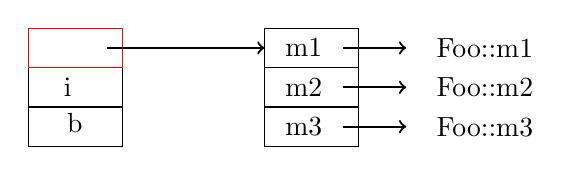
\begin{tikzpicture}
\draw (0,0)  rectangle (1.2,0.5);
\pgftext[at={\pgfpoint{0.65cm}{0.3cm}}]{b } ;
%\draw[->] (1.0, 0.1) .. controls (1.9, -0.2) and (2.5, 2.5) .. (3,1.5);

\draw (0,0.5)  rectangle (1.2,1.0);
\pgftext[at={\pgfpoint{0.5cm}{0.75cm}}]{i} ;


\draw[red] (0,1.0)  rectangle (1.2,1.5);
\pgftext[at={\pgfpoint{0.5cm}{1.25cm}}]{} ;
\draw[->, thick] (1.0, 1.25) -- (3.0,1.25); 





% right one 
\draw (3,0)  rectangle (4.2,0.5);
\pgftext[at={\pgfpoint{3.5cm}{0.25cm}}]{m3} ;
\draw[->, thick] (4.0, 0.25) -- (4.8,0.25); 
\pgftext[at={\pgfpoint{5.8cm}{0.25cm}}]{Foo::m3} ;

\draw (3,0.5)  rectangle (4.2,1.0);
\pgftext[at={\pgfpoint{3.5cm}{0.75cm}}]{m2} ;
\draw[->, thick] (4.0, 0.75) -- (4.8,0.75); 
\pgftext[at={\pgfpoint{5.8cm}{0.75cm}}]{Foo::m2} ;

\draw (3,1.0)  rectangle (4.2,1.5);
\pgftext[at={\pgfpoint{3.5cm}{1.25cm}}]{m1} ;
\draw[->, thick] (4.0, 1.25) -- (4.8,1.25); 
\pgftext[at={\pgfpoint{5.8cm}{1.25cm}}]{Foo::m1} ;

\end{tikzpicture}
}
\end{tabular}

\end{tabular}
\end{frame}




\begin{frame}[fragile]
\frametitle{Virtual function table and inheritance}
\framesubtitle{}
\begin{tabular}{ll}
\begin{minipage}{4.3cm}
\begin{cplus3}
class Foo {
  int i;
  boolean b;
  public void m1() {...}
  public Integer m2() {...}
  public Window m3() {..}
}
class Bar extends Foo {
  int y;

  // override
  public void m1() {..}

  // extend
  public int m4() {..}
}
Bar b = new Bar();
\end{cplus3}
\end{minipage}

& 

\begin{tabular}{l}
{\small 
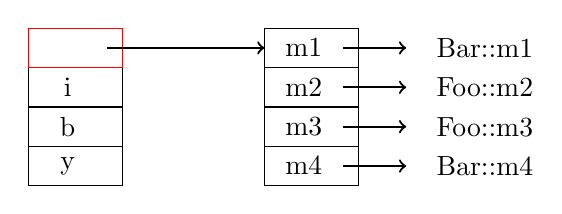
\begin{tikzpicture}

\draw (0,-0.5)  rectangle (1.2,0.0);
\pgftext[at={\pgfpoint{0.5cm}{-0.25cm}}]{y} ;

\draw (0,0)  rectangle (1.2,0.5);
\pgftext[at={\pgfpoint{0.5cm}{0.25cm}}]{b} ;


\draw (0,0.5)  rectangle (1.2,1.0);
\pgftext[at={\pgfpoint{0.5cm}{0.75cm}}]{i} ;


\draw[red] (0,1.0)  rectangle (1.2,1.5);
\pgftext[at={\pgfpoint{0.5cm}{1.25cm}}]{} ;
\draw[->, thick] (1.0, 1.25) -- (3.0,1.25); 





% right one 
\draw (3,-0.5)  rectangle (4.2,0.0);
\pgftext[at={\pgfpoint{3.5cm}{-0.25cm}}]{m4} ;
\draw[->, thick] (4.0, -0.25) -- (4.8,-0.25); 
\pgftext[at={\pgfpoint{5.8cm}{-0.25cm}}]{Bar::m4} ;


\draw (3,0)  rectangle (4.2,0.5);
\pgftext[at={\pgfpoint{3.5cm}{0.25cm}}]{m3} ;
\draw[->, thick] (4.0, 0.25) -- (4.8,0.25); 
\pgftext[at={\pgfpoint{5.8cm}{0.25cm}}]{Foo::m3} ;

\draw (3,0.5)  rectangle (4.2,1.0);
\pgftext[at={\pgfpoint{3.5cm}{0.75cm}}]{m2} ;
\draw[->, thick] (4.0, 0.75) -- (4.8,0.75); 
\pgftext[at={\pgfpoint{5.8cm}{0.75cm}}]{Foo::m2} ;

\draw (3,1.0)  rectangle (4.2,1.5);
\pgftext[at={\pgfpoint{3.5cm}{1.25cm}}]{m1} ;
\draw[->, thick] (4.0, 1.25) -- (4.8,1.25); 
\pgftext[at={\pgfpoint{5.8cm}{1.25cm}}]{Bar::m1} ;

\end{tikzpicture}
}
\end{tabular}

\end{tabular}
\end{frame}

\begin{frame}[fragile]
\frametitle{Evaluation}
\framesubtitle{}
Advantage of polymorphic methods: 
\begin{itemize}
\item Flexibility: the ``most specific'' method is called
(namely the one defined for the actual type)
\item Major motivation for using OOP
\end{itemize}
\bigskip

Disadvantage of polymorphic methods: 
\begin{itemize}
\item Expensive: run-time overhead due to dynamic dispatch
\item No inlining possible $\leadsto$ many compiler optimizations
impossible
\end{itemize}

\end{frame}





\section{Multiple Inheritance}

\begin{frame}[fragile]
\frametitle{Motivation}
\framesubtitle{}
Consider the following classes (cp. Smalltalk)
\begin{itemize}
\item Magnitude: for objects that are measurable (comparable)
\item Number: for objects that are measurable and have arithmetics
\end{itemize}
Assume you want to add the classes Char, Integer, and Complex.
Constraints
\begin{itemize}
\item Char should be subclass of Magnitude, but not of Number.
\item Integer should be subclass of Magnitude and Number.
\item Complex should be a subclass of Number, but not of Magnitude.
\end{itemize}
Impossible with single inheritance.
\end{frame}

\begin{frame}[fragile]
\frametitle{Limitations of single inheritance}
\framesubtitle{}
Workarounds for the previous example:

\begin{itemize}
\item Limit inheritance: eliminate class Magnitude; every measurable
class implements its comparisons
\item Violate substitutability: define Complex as subclass of Number
(and Number as subclass of Measurable), but override measurable
methods so that they trigger error.
\item Avoid inheritance: define each method in each of the classes
Char, Integer, Complex.
\end{itemize}
\end{frame}

\begin{frame}[fragile]
\frametitle{Multiple inheritance}
\framesubtitle{}
In \textit{multiple inheritance}, a class may inherit from one or
more superclasses.
\bigskip

Languages
\begin{itemize}
\item Most OO languages support single inheritance only.
\item Eiffel, \cpp, CLOS support multiple inheritance.
\item Java, C\# support mix-in inheritance (``interfaces''). 

\end{itemize}
\end{frame}

\begin{frame}[fragile]
\frametitle{Object model under multiple inheritance}
\framesubtitle{}
\begin{tabular}{ll}
\begin{minipage}{4.3cm}
\begin{cplus3}
class Person
{ 
   int p1;
   int& p2;
   boolean p3; 
   virtual void m1(..) {...}
   virtual int m2(..) {...}  
};
class Student 
{
   char s1;
   char s2;
};
class Asst : Person, Student 
{
    int a1;
};
\end{cplus3}
\end{minipage}

& 

\begin{tabular}{l}
{\small 
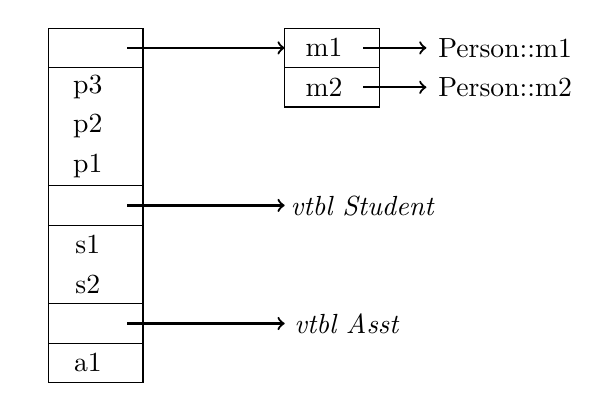
\begin{tikzpicture}

% object 3
\draw (0,-2.5)  rectangle (1.2,-3.0);
\pgftext[at={\pgfpoint{0.5cm}{-2.75cm}}]{a1} ;

% vptr object 3
\draw (0,-2.5)  rectangle (1.2,-2.0);
\pgftext[at={\pgfpoint{0.5cm}{-2.25cm}}]{} ;
\draw[->, thick] (1.0, -2.25) -- (3.0,-2.25); 
\pgftext[at={\pgfpoint{3.8cm}{-2.25cm}}]{\textit{vtbl Asst}} ;

% object 2
\draw (0,-2.0)  rectangle (1.2,-1.0);
\pgftext[at={\pgfpoint{0.5cm}{-1.25cm}}]{s1} ;
\pgftext[at={\pgfpoint{0.5cm}{-1.75cm}}]{s2} ;

% vptr
\draw (0,-1.0)  rectangle (1.2,-0.5);
\pgftext[at={\pgfpoint{-0.25cm}{-0.75cm}}]{} ;
\draw[->, thick] (1.0, -0.75) -- (3.0,-0.75); 
\pgftext[at={\pgfpoint{4.0cm}{-0.75cm}}]{\textit{vtbl Student}} ;

% object 1
\pgftext[at={\pgfpoint{0.5cm}{-0.25cm}}]{p1} ;
\pgftext[at={\pgfpoint{0.5cm}{0.25cm}}]{p2} ;
\pgftext[at={\pgfpoint{0.5cm}{0.75cm}}]{p3} ;
\draw (0,-0.5)  rectangle (1.2,1.5);

% vptr 
\draw (0,1.0)  rectangle (1.2,1.5);
\pgftext[at={\pgfpoint{0.5cm}{1.25cm}}]{} ;
\draw[->, thick] (1.0, 1.25) -- (3.0,1.25); 





% right one 

% vtbl for 

% vtbl for Person
%\draw (3,-0.5)  rectangle (4.2,0.0);
%\pgftext[at={\pgfpoint{3.5cm}{-0.25cm}}]{m4} ;
%\draw[->, thick] (4.0, -0.25) -- (4.8,-0.25); 
%\pgftext[at={\pgfpoint{5.8cm}{-0.25cm}}]{Person::m4} ;


%\draw (3,0)  rectangle (4.2,0.5);
%\pgftext[at={\pgfpoint{3.5cm}{0.25cm}}]{m3} ;
%\draw[->, thick] (4.0, 0.25) -- (4.8,0.25); 
%\pgftext[at={\pgfpoint{5.8cm}{0.25cm}}]{Person:m3} ;

\draw (3,0.5)  rectangle (4.2,1.0);
\pgftext[at={\pgfpoint{3.5cm}{0.75cm}}]{m2} ;
\draw[->, thick] (4.0, 0.75) -- (4.8,0.75); 
\pgftext[at={\pgfpoint{5.8cm}{0.75cm}}]{Person::m2} ;

\draw (3,1.0)  rectangle (4.2,1.5);
\pgftext[at={\pgfpoint{3.5cm}{1.25cm}}]{m1} ;
\draw[->, thick] (4.0, 1.25) -- (4.8,1.25); 
\pgftext[at={\pgfpoint{5.8cm}{1.25cm}}]{Person::m1} ;

\end{tikzpicture}
}
\end{tabular}

\end{tabular}

\end{frame}

\begin{frame}[fragile]
\frametitle{Name clashes (again)}
\framesubtitle{}
If two base classes define a method (field) with the same signature,
the ambiguity must be resolved. 

\begin{itemize}
\item Language-defined priorities
\begin{itemize}
\item CLOS: first-fit
\end{itemize}
\item Prohibited (and checked)
\begin{itemize}
\item Eiffel: error at compile time of the child class
\item Must be resolved manually, e.g., via \texttt{rename}; % or \texttt{select} 
\begin{eiffel}
class COURSE_ASSISTANT
inherit
      STUDENT
          rename
              name as teacher_name
          end
      PERSON
\end{eiffel}
\end{itemize}
\item Ambiguous use prohibited (and checked)
\begin{itemize}
\item \Cpp: no error at class compilation time, but at method invocation
time (statically)
\item Must be resolved manually,  via scope resolution operator
\begin{cplus3}
if (...) person::name() else student::name(); 
\end{cplus3} 
\end{itemize}
\end{itemize}
       select 
          move ..

\end{frame}


\begin{frame}[fragile]
\frametitle{Repeated inheritance}
\framesubtitle{}
In \textit{repeated}  inheritance, a class serves as 
ancestor repeatedly, through multiple inheritance relationships. 

\begin{cplus3}
class A;
class B: public A {...}
class C: public A {.. }
class D: public B, C {...}
\end{cplus3}

Replicated: 
\begin{itemize}
\item  $D$ objects contain 2 copies of $A$ objects
\item \Cpp's default choice. Shared inheritance requires keyword \texttt{virtual}.
\end{itemize}
Shared (``diamond''): 
\begin{itemize}
\item  $D$ objects contain only 1 $A$ object.
\item Eiffel's choice. Replication inheritance only via renaming. 
\end{itemize}

\end{frame}

\begin{frame}[fragile]
\frametitle{Replicated inheritance}
\framesubtitle{}
Default case in \Cpp. 
\begin{cplus3}
class A;
class B: public A {...}
class C: public A {.. }
class D: public B, C {...}
\end{cplus3}


\begin{itemize}
\item Members of $A$ are ambiguous $\leadsto$ no direct access possible
(scope resolution operator doesn't help); access via parents needed.  
\item Virtual function tables are merged  and the portions $C::A$ methods
and $B::A$ methods are kept. 

\mycomment{
\begin{cplus3}
// C++ 
A* b; B* b; C* c; D* d;
a = d; // error
b = d; 
c = d;
a = b;
a = c; 
\end{cplus3}
}
\end{itemize}
\bigskip

Problem: inconsistency
\end{frame}

\begin{frame}[fragile]
\frametitle{Shared inheritance}
\framesubtitle{}
Default case in Eiffel. In \cpp, the keyword \texttt{virtual} 
indicates sharing.
Shared inheritance avoids name clashes between parents.

\begin{cplus3}
class A;
class B: public virtual A {...}
class C: public virtual A {.. }
class D: public B, C {...}
\end{cplus3}



New ambiguity: what if both $B$ and $C$ override a method in $A$?
\begin{itemize}
\item Eiffel: use \texttt{select} to resolve ambiguity
\item \Cpp: compile-time error
\end{itemize}

General problem:


\begin{itemize}
\item In \Cpp, neither child nor virtual parent determine the construction
of parent objects---only grandchildren.
%\item In \Cpp, virtual function table gets either bigger or there is an additional level of indirection.
\item In Eiffel, it depends on the future client whether
a feature will be shared or replicated.
\end{itemize}
$\leadsto$ Implementation quite 
complicated 
\end{frame}

\begin{frame}[fragile]
\frametitle{Mix-in inheritance and interface}
\framesubtitle{}
\textit{Mix-in inheritance} is an alternative to multiple inheritance, but
avoids problems or complications with replicated inheritance.

\begin{itemize}
\item Same motivation: combine \textit{orthogonal} functionality
\item Encapsulate each functionality in a class
\item No superclasses: mix-in classes are in
flat hierarchies 
\item No subclasses:  a mix-in class is for
``mixing in'' properties and cannot be instantiated
\end{itemize}

Example: interfaces in Java and C\#
\end{frame}

\end{document}


\begin{frame}[fragile]
\frametitle{Design by contract in Eiffel}
\framesubtitle{http://archive.eiffel.com/doc/online/eiffel50/intro/language/tutorial-09.html}
The contract of a class contains pre- and postconditions and class invariants.
\begin{cplus3}
indexing
    description: "Simple bank accounts"
class interface
    ACCOUNT
feature -- Access
    balance: INTEGER
            -- Current balance
    deposit_count: INTEGER
            -- Number of deposits made since opening
feature -- Element change
    deposit (sum: INTEGER)
            -- Add sum to account.
         require
            non_negative: sum >= 0
         ensure
            one_more_deposit: deposit_count = old deposit_count + 1
            updated: balance = old balance + sum
invariant
    consistent_balance: balance = all_deposits . total
end -- class interface ACCOUNT
\end{cplus3}
\end{frame}


